%\graphicspath{{/home/arbon/Pictures/Screenshots/}} % path to graphics
\graphicspath{{~/Documents/SADT/FirstTask/RMS}}
\chapter{Системы управления репозиториями}

\section{Создание репозитория на GitHub и на локальной машине}
\subsection{Создание репозитория на GitHub}
Чтобы создать репозиторий в GitHub, нужно:
\begin{enumerate}
	\item Перейти во вкладку "<repositories">.
	\item Нажать на кнопу "<New">.
	\item Ввести название для репозитория и нажать кнопку.
\end{enumerate}
Окно создания репозиторя изображено на рисунке \ref{2:fig:GitHub:create_repo}.
\begin{figure}[h!tp]
	\centering
	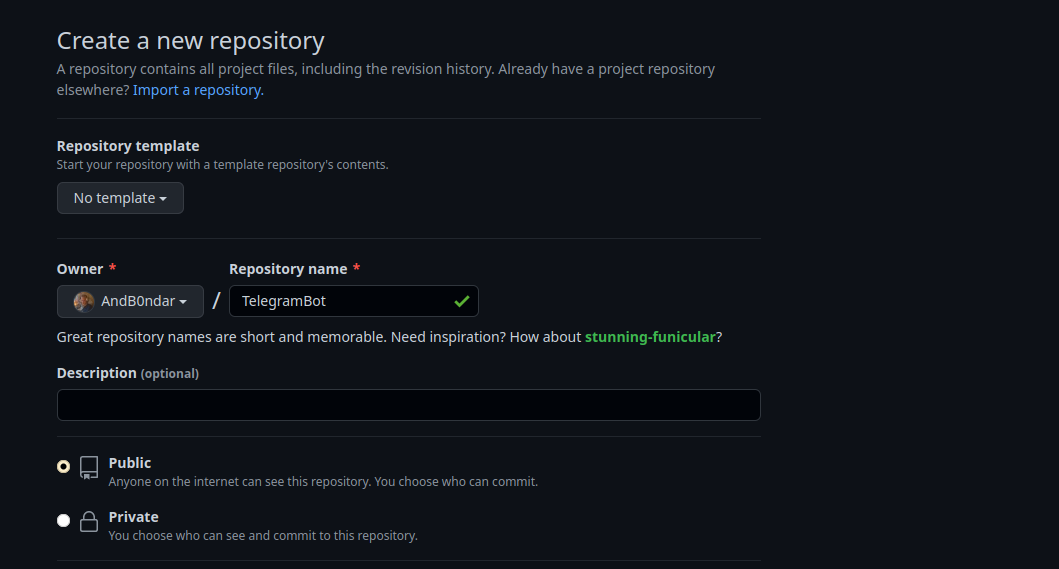
\includegraphics[width=0.8\textwidth]{Screenshot from 2023-02-19 16-04-27.png}
	\caption{Создание репозитория в GitHub}
	\label{2:fig:GitHub:create_repo}
\end{figure}

\section{Создание репозитория на локальной машине}
Создание репозитория рассматривалось в прошлой части. Так что опишем вкратце:
\begin{enumerate}
	\item Создадим каталог, где будет размещаться репозиторий.
	\item Добавим файлы в каталог.
	\item Создадим локальный репозиторий, командой~\texttt{git~init}.
	\item Добавим файлы в индекс, комнадой~\texttt{git~add~<файлы>}.
	\item Сделаем коммит, чтобы сохранить изменнения в репозиторий,
		командой \texttt{git~commit~-m~"текст~коммита"}.
\end{enumerate}
Консольный вывод показан на рисунке \ref{2:fig:git:init}.
\begin{figure}[h!tp]
	\centering
	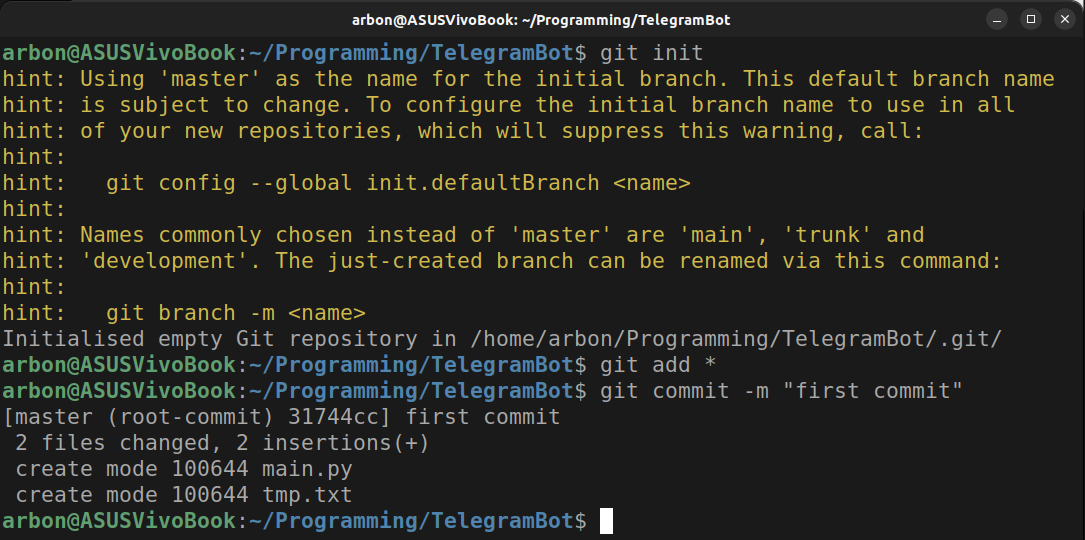
\includegraphics[width=0.8\textwidth]{Screenshot from 2023-02-19 16-38-18.png}
	\caption{Создание репозитория в GitHub}
	\label{2:fig:git:init}
\end{figure}

\section{Создание SSH-ключа}
Чтобы работать со своего компьютера с GitHub, иметь доступ к проектам,
хранящимся на сервисе, выполнять команды в консоли без постоянного
подтверждения пароля, нужно пройти авторизацию у сервера.
В этом помогают SSH-ключи.

Для создания ключа нужно воспользоваться командой:
\begin{verbatim}
	ssh-keygen -t rsa -b 4096 -C "your_email@example.com"
\end{verbatim}

Во время работы команды потребуется ввести: путь, по которому будет
располагаться созданный ключ, и пароль к создаваемому ключу.
Обычно ключи сохраняются в кталоге .ssh домашней директории. Его содержимое
отображено на рисунке~\ref{2:fig:ssh-key}.

\begin{figure}[h!tp]
	\centering
	
\includegraphics[width=0.8\textwidth]{Screenshot from 2023-02-19 16-45-31.png}
	\caption{Каталог с созданными ssh ключами}
	\label{2:fig:ssh-key}
\end{figure}

\section{Связывание локального и GitHub репозитория}
Для того, чтобы связать репозиторий на локальной машине и созданным выше
удаленный репозиторием, вначале необходимо зарегестрировать
наш ssh ключ в GitHub. Мы должны его скопировать из консоли
и перейти на страницу для работы с ключами в профиле на GitHub.
Выбираем кнопку “New SSH key”, открывается окно с вводом данных, в поле “key”
вставляем скопированный ключ, в “Title” вводим любое
имя ключа и нажимаем “Add SSH key”.
Добавленный ключ показан на рисунку \ref{2:fig:GitHub:add_ssh-key}
\begin{figure}[h!tp]
	\centering
	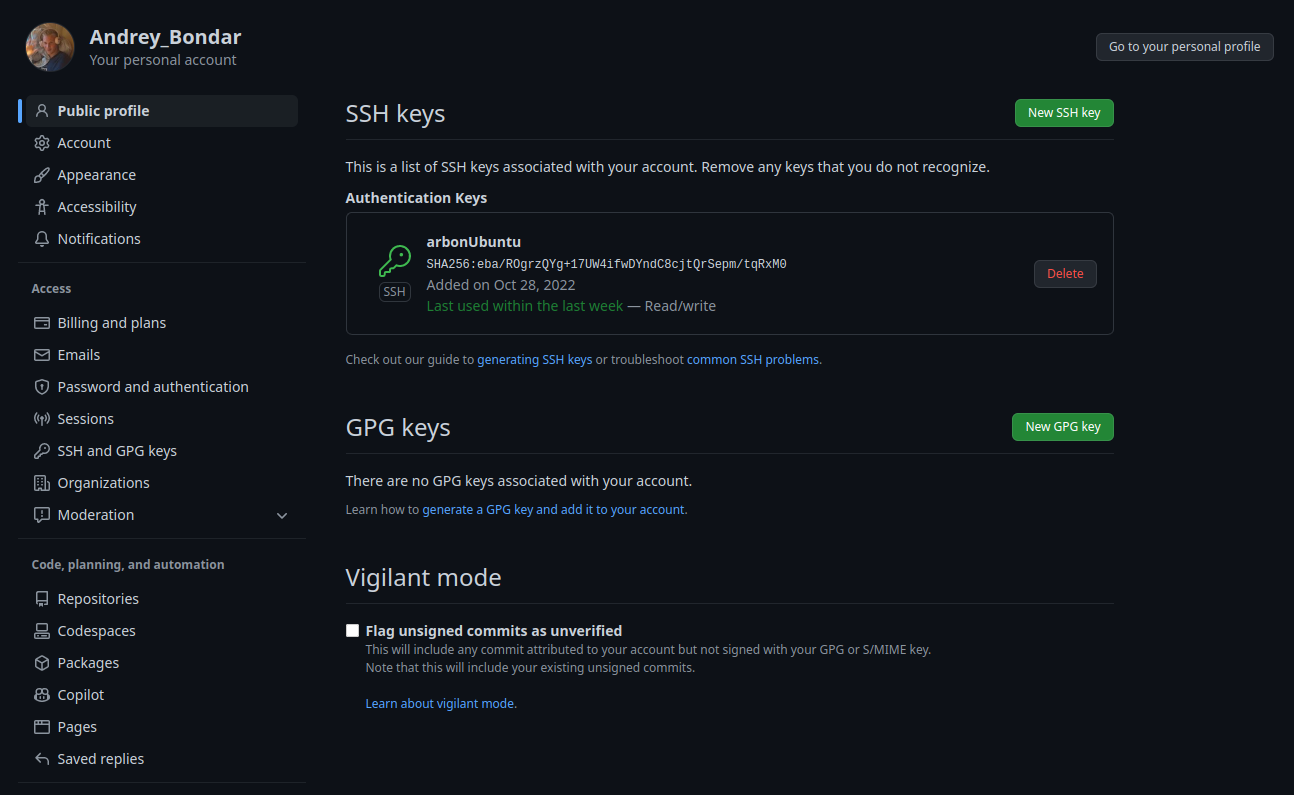
\includegraphics[width=0.8\textwidth]{Screenshot from 2023-02-19 17-08-36.png}
	\caption{Добавленный ssh-ключ в GitHub}
	\label{2:fig:GitHub:add_ssh-key}
\end{figure}

Чтобы связать локальный и удаленный репозитории друг с другом необходимо
ввести в консоль следующую команду:
\begin{verbatim}
	git remote add project \
		git@github.com:<ваши имя и название репозитория>.git
	git branch -M main
	git push -u origin main
\end{verbatim}
Вывод команд показан на рисунке~\ref{2:fig:git:remote}.
\begin{figure}[h!tp]
	\centering
	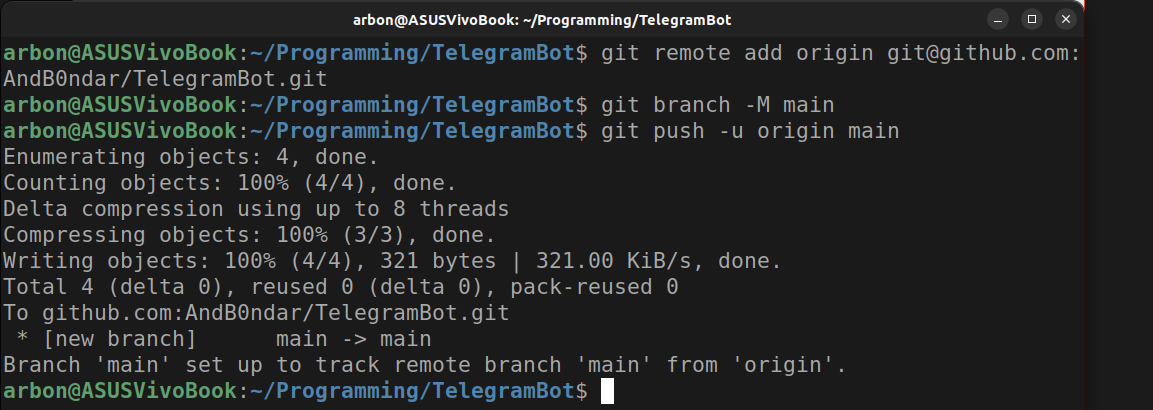
\includegraphics[width=0.8\textwidth]{Screenshot from 2023-02-19 17-16-49.png}
	\caption{Связывание репозиториев}
	\label{2:fig:git:remote}
\end{figure}

\section{Создание и слияние новой ветки}
Создание новой ветки в git выполняется
командой: \texttt{git~branch~<имя~ветки>}.

Чтобы изменить текущую ветку есть команда: \texttt{git~checkout~<имя~ветки>}.

Эти две команды можно объединить, чтобы создать новую ветки и сразу на нее переключиться: \texttt{git~checkout~-b~<имя~ветки>}.

Чтобы слить вде ветки, нужно перейти в ту ветку в которую нужно объединить изменения и ввести команду: \texttt{git~merge~<название~ветки>}, как показано
на рисунке \ref{2:fig:git:merge}.

\begin{figure}[h!tp]
	\centering
	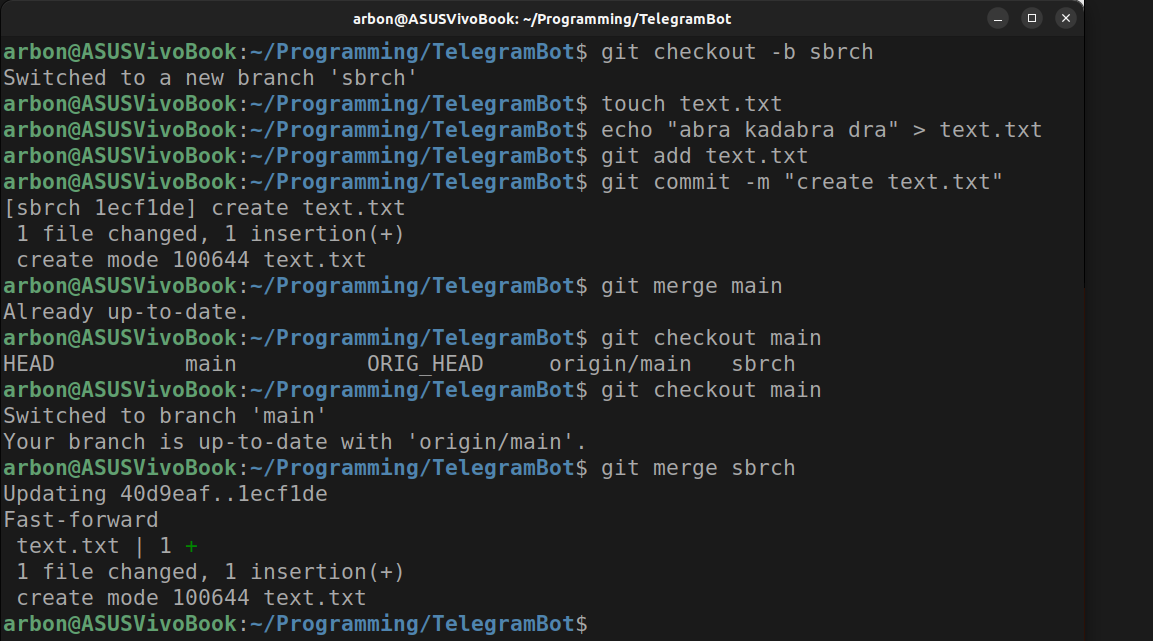
\includegraphics[width=0.8\textwidth]{Screenshot from 2023-02-19 17-34-01.png}
	\caption{Слияние веток в git}
	\label{2:fig:git:merge}
\end{figure}

\section{Задание варианта}
Выполним цепочку действий в репозитории, согласно 3-ему варианту:
\begin{itemize}
	\item Клонируем непустой удаленный репозиторий на локальную
		машину (Рисунок \ref{2:fig:git:clone}).
		\begin{figure}[h!tp]
			\centering
			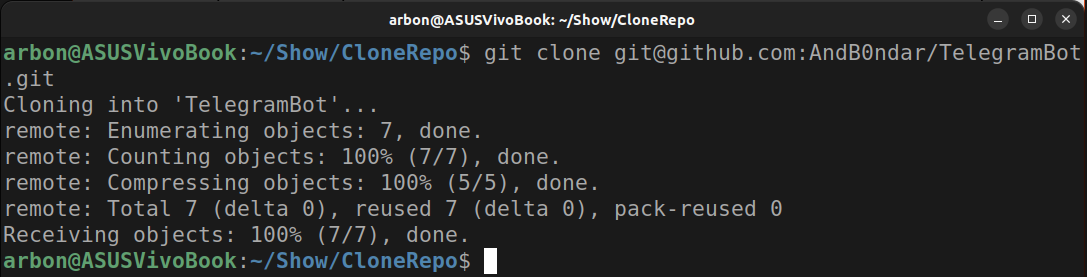
\includegraphics[width=0.8\textwidth]{Screenshot from 2023-02-19 17-49-39.png}
			\caption{Клонирование удаленного репозиторя}
			\label{2:fig:git:clone}
		\end{figure}

	\item Создадим тег указывающий на последний коммит
		в ветке master(Рисунок \ref{2:fig:git:tag-branch}).
	\item Создадим новую ветку и выведите список
		всех веток (Рисунок \ref{2:fig:git:tag-branch}).
		\begin{figure}[h!tp]
			\centering
			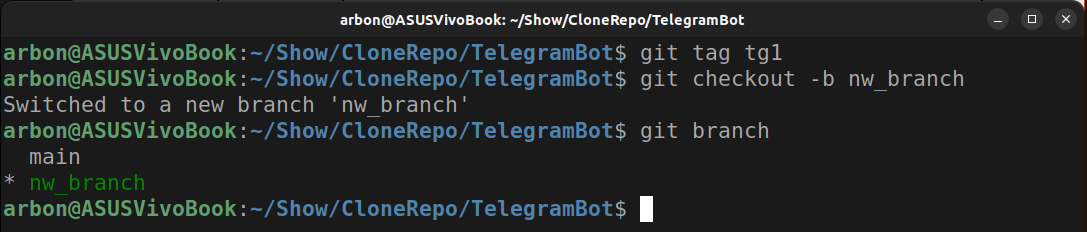
\includegraphics[width=0.8\textwidth]{Screenshot from 2023-02-19 17-54-18.png}
			\caption{Создание тега и новой ветки}
			\label{2:fig:git:tag-branch}
		\end{figure}

	\item Произведем 3 коммита в новой ветке
		(Рисунок \ref{2:fig:git:three_commits}).
		\begin{figure}[h!tp]
			\centering
			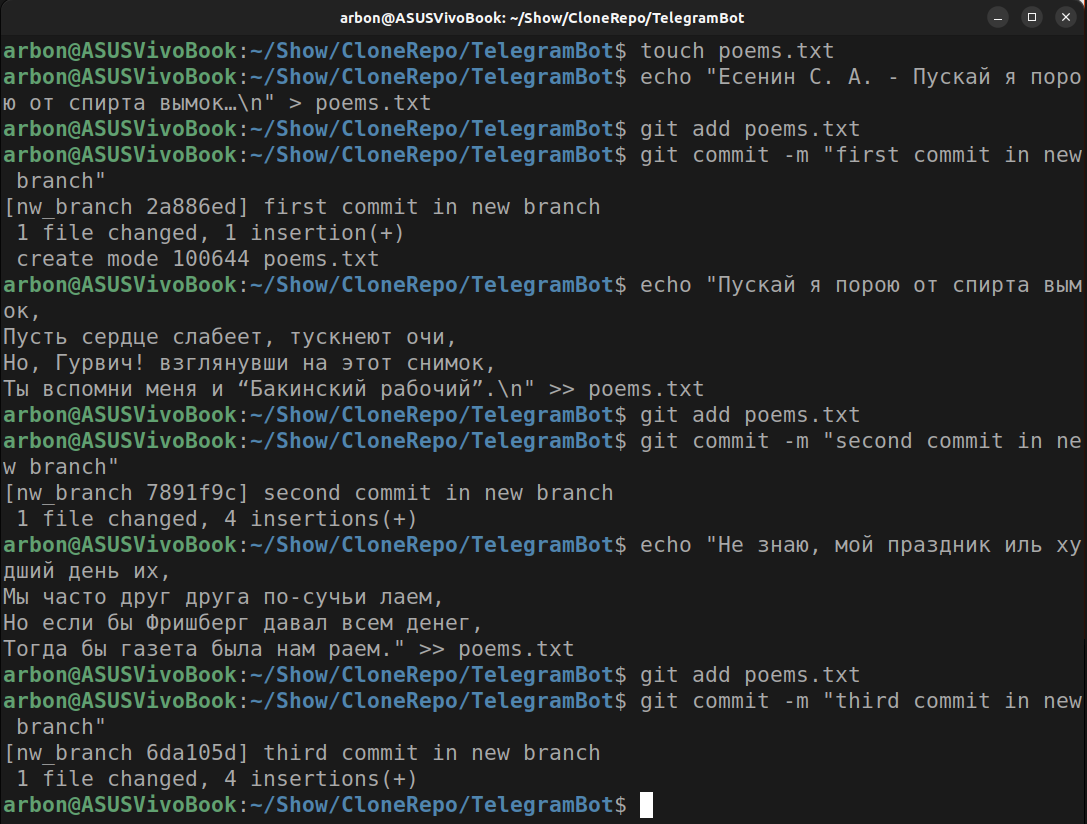
\includegraphics[width=0.8\textwidth]{Screenshot from 2023-02-19 18-02-24.png}
			\caption{Создание трех коммитов}
			\label{2:fig:git:three_commits}
		\end{figure}

	\item Выгрузим все изменения в удаленный
		репозиторий (Рисунок \ref{2:fig:git:push}).
		\begin{figure}[h!tp]
			\centering
			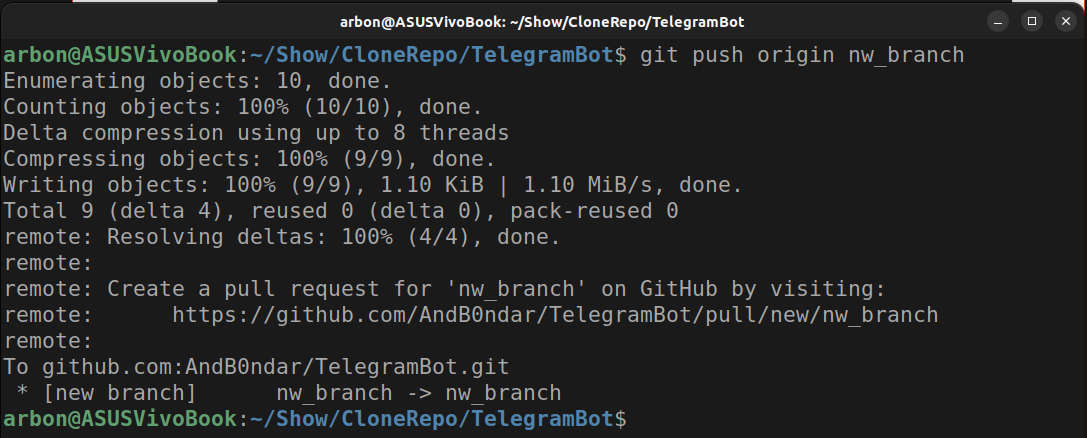
\includegraphics[width=0.8\textwidth]{Screenshot from 2023-02-19 18-06-52.png}
			\caption{Отправка изменений в удаленный репозиторий}
			\label{2:fig:git:push}
		\end{figure}

	\item Откатим ветку к созданному тегу
		(в том числе в удаленном репозитории)
		(Рисунок \ref{2:fig:git:checkout}).
		\begin{figure}[h!tp]
			\centering
			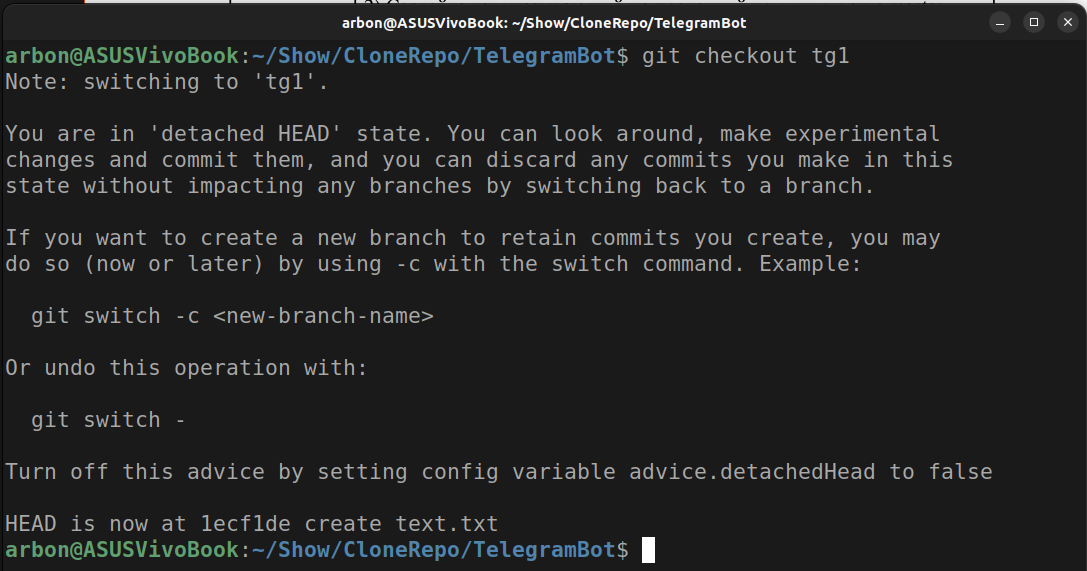
\includegraphics[width=0.8\textwidth]{Screenshot from 2023-02-19 18-20-49.png}
			\caption{Откатка ветки к созданному тегу}
			\label{2:fig:git:checkout}
		\end{figure}

	\item Выведим в консоли различия между веткой master
		и новой веткой (Рисунок \ref{2:fig:git:diff}).
		\begin{figure}[h!tp]
			\centering
			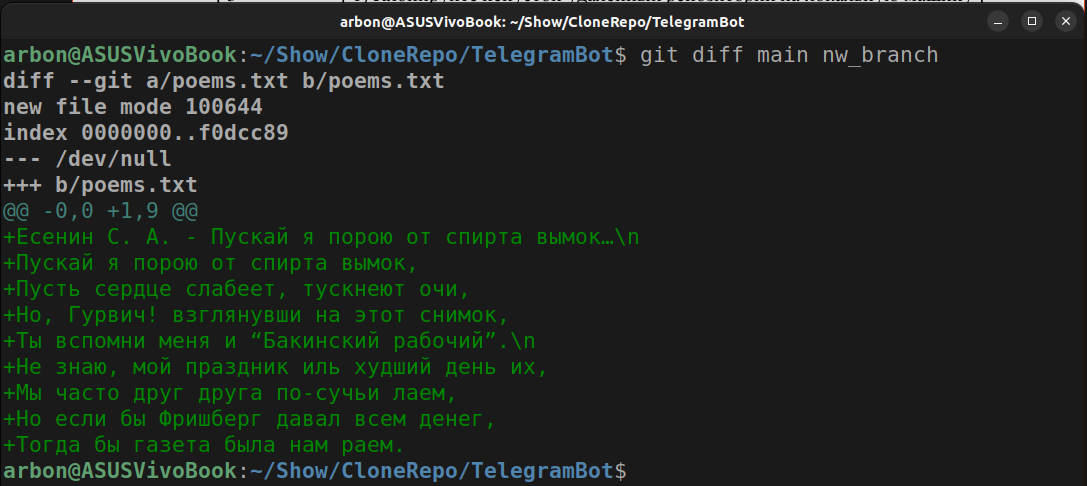
\includegraphics[width=0.8\textwidth]{Screenshot from 2023-02-19 18-13-02.png}
			\caption{Различия между ветками}
			\label{2:fig:git:diff}
		\end{figure}
\end{itemize}
